\pdfoutput=1
\documentclass[10pt, logo, twocolumn, copyright, nonumbering]{nvidiatechreport}

\usepackage{hyperref}
\usepackage{url}
\usepackage{colortbl}
\usepackage{nicefrac}       %
\usepackage{microtype}      %
\usepackage[dvipsnames]{xcolor}         %
\usepackage{multirow}
\usepackage{multicol}
\usepackage{graphicx}
\usepackage{xspace}
\usepackage{amsmath}
\usepackage{adjustbox}
\usepackage{tcolorbox}
\usepackage{amssymb}
\usepackage{enumitem}
\usepackage{wrapfig}
\usepackage{xcolor}
\usepackage{subcaption}    %
\usepackage{float}
\usepackage{stfloats}
\usepackage{amsmath}
\usepackage{listings}
\usepackage{mdframed}
\usepackage{tcolorbox}
\usepackage{arydshln}
\usepackage{booktabs} 
\usepackage{color,soul}
\usepackage[numbers]{natbib}

\tcbuselibrary{listings,breakable}

\definecolor{pastelblue}{RGB}{173,216,230}
\definecolor{pastelyellow}{RGB}{255,253,208}
\definecolor{pastelpink}{RGB}{255,209,220}
\definecolor{pastelgreen}{RGB}{176,226,172}
\definecolor{pastellavender}{RGB}{230,230,250}


\definecolor{NvidiaGreen}{RGB}{118, 185, 0}
\sethlcolor{red!15}


\newcommand{\dataset}[0]{OpenMathInstruct-2\xspace}
\newcommand{\datasize}[0]{14M\xspace}
\newcommand{\uniqquesns}[0]{600K\xspace}

\newcommand{\IG}[1]{{\color{green} [{\bf IG:} [comment] #1]}}
\newcommand{\WD}[1]{{\color{blue} [{\bf WD:} #1]}}
\newcommand{\IM}[1]{{\color{red} [{\bf IM:} #1]}}
\newcommand{\BK}[1]{{\color{brown} [{\bf BK:} #1]}}
\newcommand{\ST}[1]{{\color{purple} [{\bf ST:} #1]}}





\title{\dataset: Accelerating AI for Math with Massive Open-Source Instruction Data} 

\author{
\centering {Shubham Toshniwal, Wei Du, Ivan Moshkov, Branislav Kisacanin \hspace{1.8in}Alexan Ayrapetyan, Igor Gitman
}
}






\begin{abstract}
\textbf{Abstract:} 

Mathematical reasoning continues to be a critical challenge in large language model (LLM) development with significant interest.  
However, most of the cutting-edge progress in mathematical reasoning with LLMs has become \emph{closed-source} due to lack of access to training data. 
This lack of data access limits researchers from understanding the impact of different choices for synthesizing and utilizing the data. 
With the goal of creating a high-quality finetuning (SFT) dataset for math reasoning, we conduct careful ablation experiments on data synthesis using the recently released \texttt{Llama3.1} family of models. 
Our experiments show that: (a) solution format matters, with excessively verbose solutions proving detrimental to SFT performance, (b) data generated by a strong teacher outperforms equally-sized data generated by a weak student model, (c) SFT is robust to low-quality solutions, allowing for imprecise data filtering, and (d) question diversity is crucial for achieving data scaling gains.   
Based on these insights, we create the \dataset dataset which consists of 14M question-solution pairs ($\approx$ 600K unique questions), making it nearly eight times larger than the previous largest open-source math reasoning dataset. 
Finetuning the \texttt{Llama-3.1-8B-Base} using OpenMathInstruct-2 outperforms \texttt{Llama3.1-8B-Instruct} on MATH by an absolute 15.9\% (51.9\% $\rightarrow$ 67.8\%). 
Finally, to accelerate the open-source efforts, we release the code, the finetuned models, and the OpenMathInstruct-2 dataset under a commercially permissive license.
\end{abstract}

\begin{document}

\maketitle


\section{Introduction}
%
Large Transformers have enabled a number of breakthrough advances in modeling language, vision, audio, biology and numerous other domains \citep{vaswani2017attention}, \citep{dosovitskiy2020image}, \citep{radford2022robust}, \citep{cramer2021alphafold2}. Much of the success of Transformers, powered by the attention operator \citep{vaswani2017attention}, relies on their scaling properties \citep{hoffmann2022training} and the emergence of in-context learning \citep{garg2022can}, which allows them to generalize to unseen data and tasks given context as input. 
%
The Transformer block is a powerful tool for sequence modeling, but it is not without its limitations. One of the most notable is the computational cost, which grows rapidly as the length of the input sequence increases. Specifically, the cost scales quadratically with the length $L$ of the sequence, which places a strict limit on the amount of context that can be considered by the model.
%
Breaking the quadratic barrier is a key step towards new possibilities for deep learning, such as using entire textbooks as context, generating long-form music or processing gigapixel scale images.

Efforts to reduce the computational cost of attention in models primarily involve the use of linearized, low-rank, and sparse approximations \citep{child2019generating,wang2020linformer,kitaev2020reformer,zhai2021attention,roy2021efficient,schlag2021linear,tu2022maxvit}. These approaches introduce a trade-off between expressivity and speed, requiring hybridization with standard attention layers to reach Transformer quality \citep{mehta2022long,dao2022hungry}.

A growing amount of evidence suggests that attention mechanisms only utilize a small portion of their quadratic capabilities for language processing \citep{olsson2022context, dao2022hungry}, leading us to question its role as the gold-standard operator for deep learning at scale. Specifically, we ask:

%
\begin{figure*}[t]
    \centering
    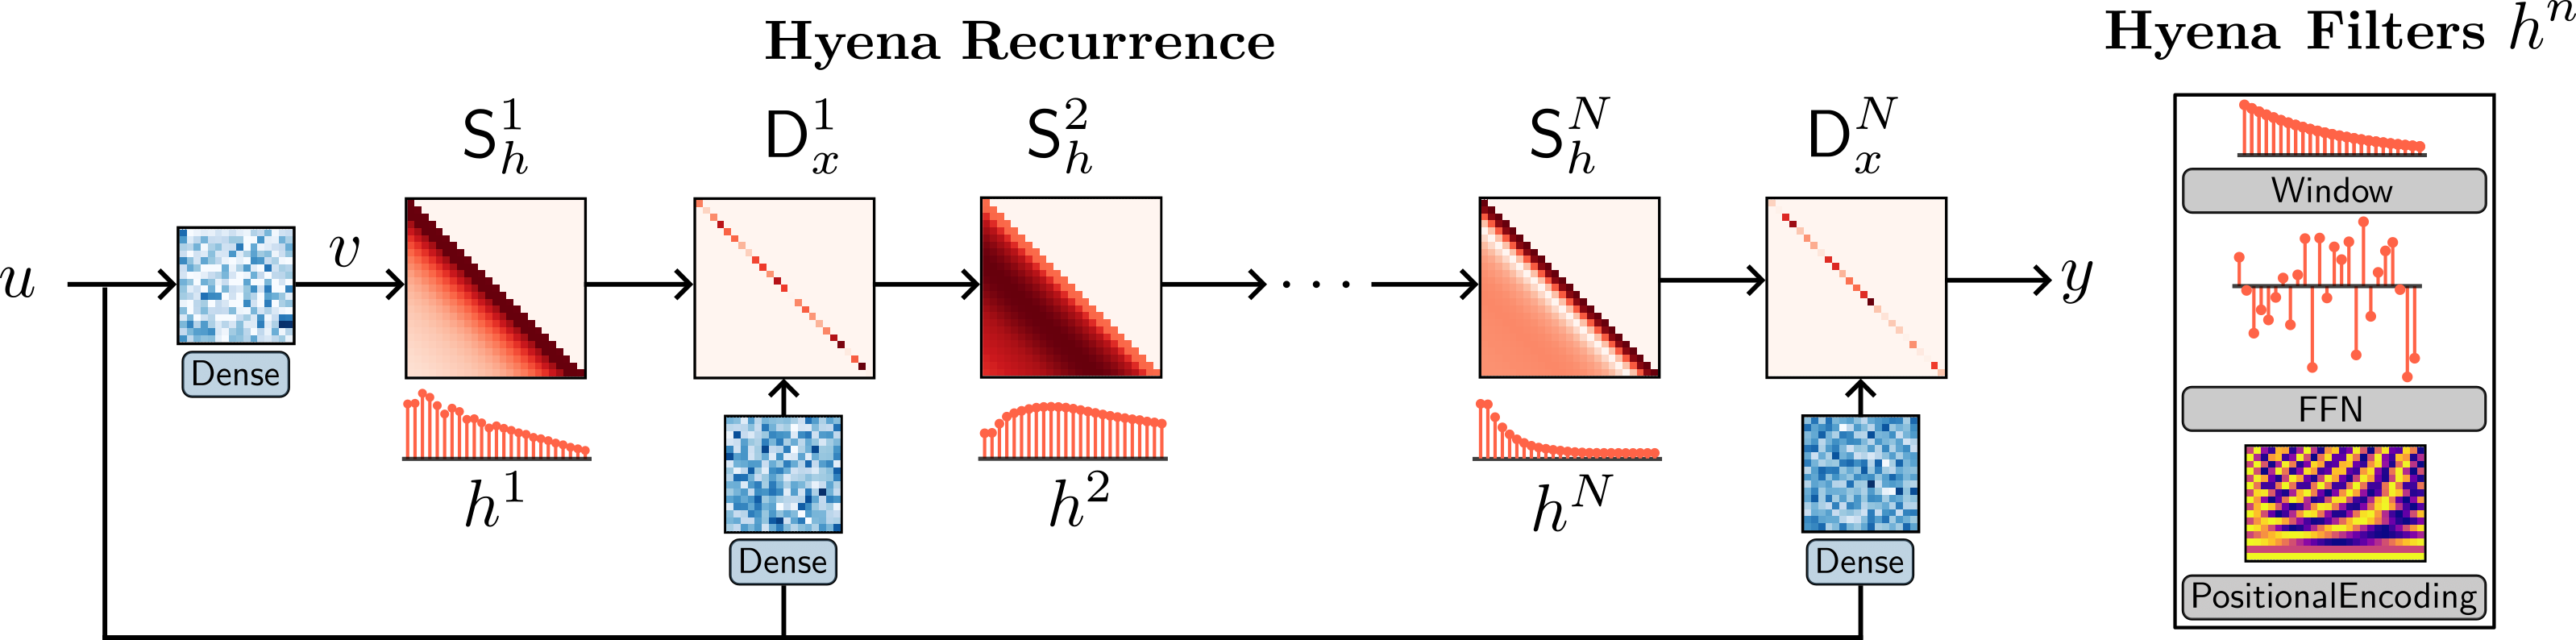
\includegraphics[width=\linewidth]{figures/hyena.png}
    \vspace{-2mm}
    \caption{The ${\sf Hyena}$ operator is defined as a recurrence of two efficient subquadratic primitives: an implicit long convolution $h$ (i.e. {\sf Hyena} filters parameterized by a feed-forward network) and multiplicative element-wise gating of the (projected) input. The depth of the recurrence specifies the size of the operator. {\sf Hyena} can equivalently be expressed as a multiplication with \textit{data-controlled} (conditioned by the input $u$) diagonal matrices $\sD_x$ and Toeplitz matrices $\sS_h$. In addition, {\sf Hyena} exhibits sublinear parameter scaling (in sequence length) and unrestricted context, similar to attention, while having lower time complexity.}
    \label{arch}
\end{figure*}
%

{\centering
\textit{Are there subquadratic operators that can match the quality of attention at scale?}\par}

\vspace{0.5cm}
% 

We obtain a positive answer based on a composition of efficient subquadratic primitives, such as \textit{element-wise multiplication} (gating) and \textit{long convolutions} i.e., convolutions with filter sizes as long as the input. We rely on a set of targeted reasoning tasks, grounded in recent work on \textit{mechanistic interpretability} \citep{elhage2021mathematical,power2022grokking,olsson2022context,zhang2022unveiling} such as recall and induction, to distill three properties of attention correlated with its performance and the quality gap with existing subquadratic approaches: 
%
\begin{itemize}[leftmargin=0.1in]
    \item[$a.$] \textbf{Data control:} Attention implements an expressive \textit{data-controlled} \citep{massaroli2020dissecting} linear operator\footnote{Self-attention can be expressed as $y = \sA(k, q) v$ where $\sA$ is the \textit{attention matrix} conditioned by linear projections $k, q$ of the input and multiplied by $v$, another projection.}, encoding an entire family of linear functions in a single block.
    \item[$b.$] \textbf{Sublinear parameter scaling:} Parameter counts of attention layers are decoupled from sequence length, allowing Transformers to allocate more parameters elsewhere e.g., the \textit{feed-forward neural networks} ({$\sf FFN$s}) between attention layers.
    \item[$c.$] \textbf{Unrestricted context:} For a given input, attention has an unrestricted context i.e., it can approximate dependencies between any two inputs, without arbitrary restrictions such as locality (except in cases using masking such as autoregressive models).
\end{itemize}
%
\paragraph{The ${\sf Hyena}$ hierarchy}
%
Guided by these findings, we introduce the ${\sf Hyena}$ hierarchy, an operator defined by a recurrence of two efficient subquadratic primitives: \textbf{a long convolution and element-wise multiplicative gating} (see Figure \ref{arch}). A specified depth (i.e., number of steps) of the recurrence controls the size of the operator. For short recurrences, existing models are recovered as special cases \citep{mehta2022long,dao2022hungry}. By mapping each step in the ${\sf Hyena}$ recurrence to its corresponding matrix form, we reveal ${\sf Hyena}$ operators to be equivalently defined as a decomposition of a \textit{data-controlled} matrix i.e., a matrix whose entries are functions of the input. Furthermore, we show how ${\sf Hyena}$ operators can be evaluated efficiently without materializing the full matrix, by leveraging fast convolution algorithms \citep{selesnick2017fast}. Empirically, ${\sf Hyena}$ operators are able to significantly shrink the quality gap with attention at scale, reaching similar perplexity and downstream performance with a smaller computational budget (Section \ref{res:lm}) and \textbf{without hybridization} of attention.
%

\paragraph{Narrowing the capabilities gap}
%
The design of {\sf Hyena} is motivated by a quality gap between standard dense attention and alternative subquadratic operators, which we identify by focusing on reasoning tasks correlated with language modeling performance at scale. We extend the suite of basic mechanistic interpretability benchmarks (\textit{induction} and \textit{recall}) with additional tasks that probe how quickly model performance degrades when task complexity increases (e.g. vocabulary size grows). In addition, we investigate the optimal parameterization of long convolutions in ${\sf Hyena}$. In the most challenging settings with hundreds of thousands of tokens, our implicit parameterization scheme improves over other operators leveraging state spaces \citep{gu2021efficiently}, frequency-domain parametrizations \citep{li2020fourier}, or standard convolutions by over $50\%$ accuracy.
%
\paragraph{Scaling in language and vision}
%
Next, we aim to verify whether rankings in our reasoning benchmark suite are predictive of quality at scale. We test ${\sf Hyena}$ on autoregressive language modeling at the sub-billion parameter scale, setting a new state-of-the-art for dense-attention-free architectures in standard datasets ({\sc WikiText103} and {\sc The Pile}) and matching Transformer quality. On the {\sc The Pile} at the $335$M parameter scale, we match Transformer perplexity with a $20\%$ reduction in the total count of \textit{floating point operations} (FLOPs). As an extension, we investigate the generality of ${\sf Hyena}$ operators by testing on large-scale image recognition, replacing attention in the Vision Transformer (ViT) \citep{dosovitskiy2020image}. In image classification, ${\sf Hyena}$ is able to match attention in accuracy when training on ImageNet-1k from scratch.
%
\paragraph{Toward much longer context}
%
Finally, we benchmark the efficiency of ${\sf Hyena}$ on long sequences. We measure $5$x speedups over dense self-attention at length $8192$ -- $2$x over highly optimized FlashAttention\footnote{FlashAttention is already 2-4x faster than a standard attention implementation in PyTorch.} \citep{dao2022flashattention} -- and $100$x speedup over FlashAttention at sequence lengths of $64$k, where standard attention implementation in PyTorch runs out of memory. 

% \vspace{-0.14in}
\section{Data: Solution Augmentation}
\label{sec:data-solution-augmentation}



In this section, we focus on the \emph{Solution Augmentation} part of the \dataset construction pipeline, shown in Figure~\ref{fig:data_overview}. 
We first give a brief overview of how solutions are synthesized for existing questions, and then present ablation studies designed to understand the impact of the different dataset design choices.  

\subsection{Solution Augmentation Preliminaries}
\label{sec:soln_augmentation}
Let $\mathcal{X} = \{\left(q_i, a_i\right)\}_{i=1}^N$ represent a 
typical mathematical reasoning dataset, where $q_i$ and $a_i$ denote the $i^\text{th}$ question and answer respectively. 
To synthesize solutions for this dataset, a \emph{teacher} LLM $\mathcal{M}$ is prompted as follows: 
$$\mathcal{I}\ \left(q_1, s_1\right), \dots, \left(q_K, s_K\right), q'$$ where $\mathcal{I}$ represents the instruction to answer the given math question, $\{q_1, \dots, q_K\}$ represent $K$ questions  representative of the dataset, $\{s_1, \dots, s_K\}$ represent their respective solutions, and $q'$ represents a question from the training set.
Given this prompt, multiple candidate solutions 
are sampled using $\mathcal{M}$. 
The high-quality solutions, usually those that lead to the correct answer, along with the prompt question $q'$, are added to the SFT dataset.



\begin{figure*}[t]
    \centering
    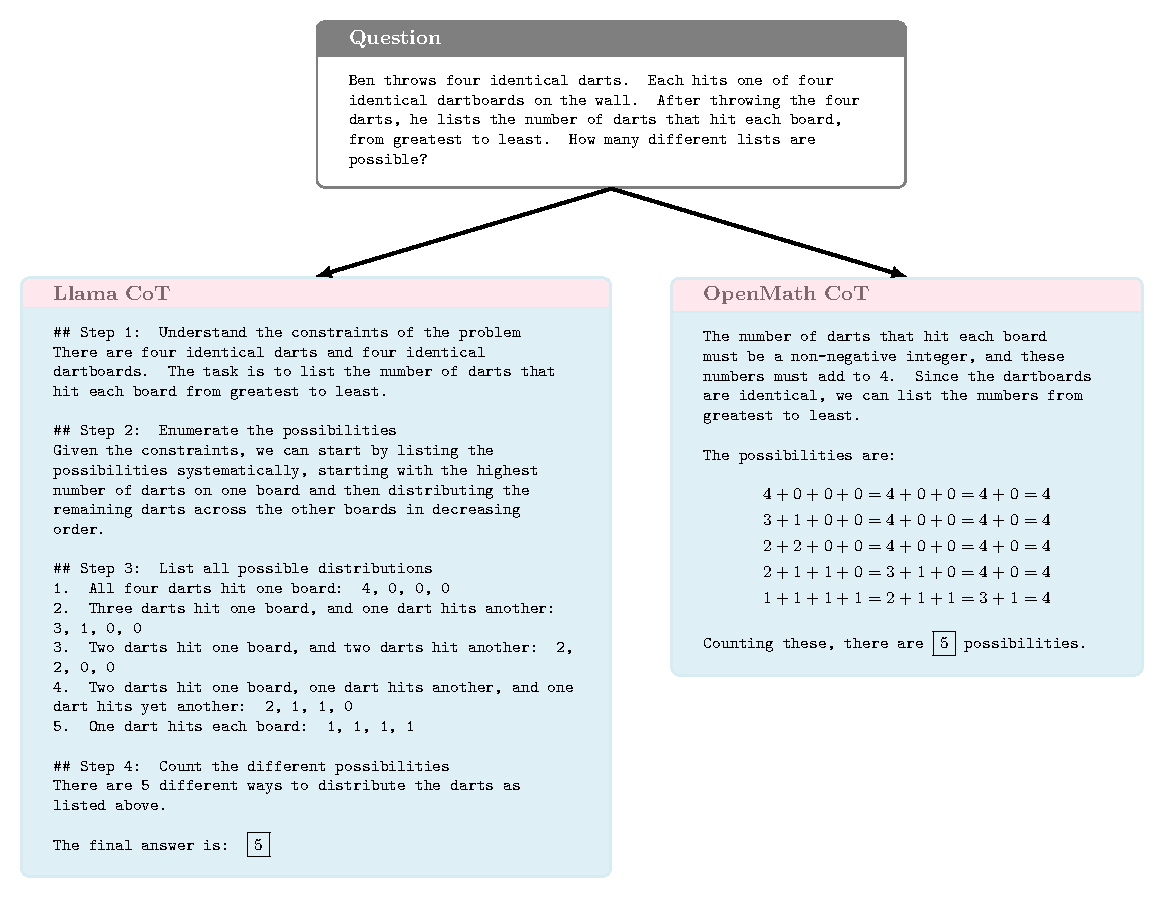
\includegraphics[width=0.95\linewidth]{figures/Solution_Format_Figure.pdf}
    \caption{A sample solution in the Llama CoT format vs.\ the OpenMath CoT format.}
    \label{fig:soln_format}
    % \vspace{-0.1in}
\end{figure*}


\subsection{Ablation Studies}
In the previous section, we gave an abstract overview of the solution augmentation pipeline. 
In practice, several design decisions impact the final SFT dataset, such as the solution format of the few-shot examples $\{s_1, \dots, s_K\}$, the choice of the teacher model $\mathcal{M}$, and the solution filtering mechanism. 
In this section, we study the impact of these different design choices on the SFT performance to guide the dataset construction. 

For these ablation experiments, we use the 1K validation split created from MATH~\citep{hendrycks2021measuringmathematicalproblemsolving} training set by \citet{toshniwal2024openmathinstruct}. The remaining 6.5K MATH training set problems are used to create the SFT dataset. 
The solutions are generated using nucleus sampling~\citep{Holtzman2020The} with a temperature of 1.0 and top-$p$ of 0.95.  
The \texttt{Llama3.1-8B-Base} model is used as the \emph{student} model in all the ablation experiments. 
For SFT, the model is trained for 4 epochs, with a batch size of 256, using the AdamW optimizer~\citep{Loshchilov2019DecoupledWD} with a constant learning rate of 5e-6 and a weight decay of 1e-2. 
To account for the variance in performance across runs, we report the performance averaged across 4 runs.   



\paragraph{Data Downsampling}
For efficiency or experiment design reasons, we sometimes need to downsize an SFT dataset to a specific size or to match another SFT dataset in ablation experiments. We introduce the concept of \emph{coverage} and the two downsampling operations used in the paper.

\emph{Coverage} of a SFT dataset $\mathcal{D}=\{\left(q_i, s_i\right)\}_{i=1}^{T}$ synthesized using dataset $\mathcal{X} = \{\left(q_i, a_i\right)\}_{i=1}^N$ is the fraction of questions in $\mathcal{X}$ with at least one solution in $\mathcal{D}$:
\[ \text{Coverage(}\mathcal{D}, \mathcal{X}\text{)} = \frac{|\{q : \left(q, s\right) \in \mathcal{D}\}|}{|\{q : \left(q, a\right) \in \mathcal{X}\}|} \]


\emph{Fair Downsampling} is a question-dependent downsampling method introduced by~\citet{toshniwal2024openmathinstruct}. 
Due to the varying difficulty of questions, the representation of ``easier'' ones can often dominate an SFT dataset, as generating high-quality solutions for them is ``easier''.  
The goal of \emph{fair} downsampling is to sample question-solution pairs from the original SFT dataset in a way that ensures all questions are as equally represented in the downsampled dataset as possible. 

\emph{Matching Coverage}:
The different design choices explored in the ablation studies result in SFT datasets of varying sizes. 
However, to compare the quality of the datasets, we want to control for the dataset size. 
To this end, we introduce the \emph{Matching Coverage} operation, where SFT datasets are matched at the level of questions. Put simply, after matching coverage, the number of unique questions as well as the number of solutions for each individual question in two dataset is the same.

Formally, suppose we're given two SFT datasets $\mathcal{D}_1$ and $\mathcal{D}_2$. 
Let $Q\left(\mathcal{D}_1\right)$ represent the set of unique questions in $\mathcal{D}_1$:
\[Q\left(\mathcal{D}_1\right) = \{q \mid \left(q, s_1\right) \in \mathcal{D}_1\}\]
The set of common questions in $\mathcal{D}_1$ and $\mathcal{D}_2$ is given by:
\[Q_{\text{match}} = Q\left(\mathcal{D}_1\right) \cap  Q\left(\mathcal{D}_2\right)\]
Let $N\left(\mathcal{D}, q\right)$ represent the number of solutions of question $q$ in dataset $\mathcal{D}$. 
In the matching coverage version of the datasets:
\[
N_\text{match}\left(q\right) = \min\left(N\left(\mathcal{D}_1, q\right), N\left(\mathcal{D}_2, q\right)\right)
\]
for each question $q \in Q_\text{match}$, $N_\text{match}\left(q\right)$ solutions are sampled from the respective datasets.  




This covers the two downsampling methods used in this paper: \emph{Fair Downsampling} and \emph{Matching Coverage}. 
Next, we will describe the ablation experiments.






\subsubsection{Solution Format}


Finetuning with synthetic chain-of-thought (CoT) solutions~\citep{nye2021workscratchpadsintermediatecomputation, wei2022chain, sprague2024cotcotchainofthoughthelps} has been the key to strong performances of small models on math reasoning tasks~\citep{yu2024metamath, toshniwal2024openmathinstruct, dubey2024llama3herdmodels}. 
We find the Llama's CoT format to be quite verbose,\footnote{\url{https://huggingface.co/datasets/meta-llama/Meta-Llama-3.1-8B-Instruct-evals/viewer/Meta-Llama-3.1-8B-Instruct-evals__math__details}} and propose an alternate CoT format, \emph{OpenMath CoT}, which is detailed as well but less verbose. 
Figure~\ref{fig:soln_format} shows a sample solution in the two CoT formats. 

\begin{table*}[t]
\setlength{\tabcolsep}{4pt}
    \centering
    \caption{Comparison of Llama and OpenMath CoT formats on MATH validation accuracy and average solution length measured in number of tokens. }
    \label{tab:soln_format}
    \begin{tabular}{lcc}
    \toprule

 &  MATH Validation Accuracy  &  Mean Solution Length  \\\midrule
Llama CoT       & 40.6 $\pm$ 0.6 & 331.3   \\
OpenMath CoT    & 44.5 $\pm$ 0.8  & 237.0  \\ 
\bottomrule 
    \end{tabular}
\end{table*}



To compare the two CoT formats, we generate SFT data using the \texttt{Llama3.1-405B-Instruct} model. 
For generating solutions in the Llama CoT format we simply use the zero-shot prompt setup as the model was trained on those kinds of solutions. 
However, even when prompting the model with few-shot OpenMath CoT solutions, a substantial number of generations -- 57\% in our experiment -- still follow the Llama CoT format. 
This tendency of \emph{aligned} models reverting to their trained behavior when encountering inputs seen during training has also been observed in prior work~\citep{min-etal-2022-rethinking}. 
We find an interesting workaround to this issue by dropping the special tokens used by Llama-Instruct models. 
Prompting the model with the ``base'' template leads to a dramatic increase in adherence to the OpenMath CoT format and reduces the Llama CoT format generations to only 0.1\%. See Appendix~\ref{sec:app_soln_format} for the prompt and more details. 







With 64 solutions sampled per question, the zero-shot setup results in about 30\% more solutions than the few-shot prompt setup (350K vs 268K). 
To control for the confounding factor of SFT data size, we perform the Matching Coverage operation over the two datasets which reduces the final SFT dataset to 260K question-solution pairs. 
Table~\ref{tab:soln_format} shows that the OpenMath CoT format is 40\% less verbose than the Llama CoT format and also results in a better SFT performance. 
All experiments presented henceforth use the OpenMath CoT format. 

    
    
    
    








\subsubsection{Choice of Teacher Model}
\label{sec:teacher_model}


Prior work has shown that with repeated sampling, even weak models can match or outperform much stronger/bigger models~\citep{li2024common7blanguagemodels, brown2024largelanguagemonkeysscaling}. 
In fact, for a fixed compute budget, a weaker model can be a better choice for a teacher model~\citep{bansal2024smallerweakerbettertraining}. 
But data synthesis is a one-time expense and a small portion of the overall compute budget of training LLMs~\citep{epoch2023tradingoffcomputeintrainingandinference}. 
We instead ask the following question: 
\emph{Can a student model learn better from its own generated solutions vs solutions generated by a strong teacher model when matching the SFT data coverage?}
\begin{table*}[t]
    \setlength{\tabcolsep}{4pt}
    \centering
    \caption{\texttt{Llama3.1-8B-Base} vs.\ \texttt{Llama3.1-405B-Instruct} as data generation models. 
    }
    \begin{tabular}{lcc}
    \toprule
        &   MATH Validation Accuracy &  Mean Solution Length \\ \midrule
    Llama3.1-8B-Base & 30.1 $\pm$ 0.6  & 205.7 \\ 
    Llama3.1-405B-Instruct & 37.9 $\pm$ 0.6 & 180.2 \\ 
    
\bottomrule 
    \end{tabular}
    \label{tab:teacher_model}
    % \vspace{-0.1in}
\end{table*}


In this ablation, we compare \texttt{Llama3.1-8B-Base} and \texttt{Llama3.1-405B-Instruct} as teacher models.  
We sample solutions using the two models and perform the Matching Coverage operation to match the final SFT datasets precisely. 
The SFT results presented in Table~\ref{tab:teacher_model}  show that even when controlling for the SFT data size, \texttt{Llama3.1-405B-Instruct} is a far superior data generation model. 
Our preliminary analysis suggests that the reason is weaker models generate more  \emph{noisy solutions} that use incorrect reasoning yet end up with the right answer and, ultimately, part of the SFT dataset (Appendix~\ref{sec:app_noisy_solutions}).  
We leave a more detailed analysis regarding this for future work.  
Next, we investigate the impact of these \emph{noisy solutions} among solutions generated by \texttt{Llama3.1-405B-Instruct}. 




\subsubsection{Impact of Low-Quality Solutions}
\label{sec:impact-of-noise}
\begin{table*}[!ht]
    \centering
    \caption{SFT performance on the MATH validation set with various filtering strategies to remove solutions with incorrect reasoning.}
    \label{tab:nosiy-data-sft-performance}
    \begin{tabular}{lcc}
    \toprule
     Filtering Strategy    &  Data Size & MATH Validation Accuracy \\ \midrule
     Unfiltered      & 128K &  43.6 $\pm$  1.7 \\
     LLM-as-a-Judge: Prompt 1 & 113K           &  43.6 $\pm$ 0.1 \\ 
     LLM-as-a-Judge: Prompt 2  & 116K          &  43.0 $\pm$
     0.8  
     \\
     Nemotron-4-340B-Reward: Helpfulness $\ge 3$             &  118K &  43.8 $\pm$ 0.4 \\
     Nemotron-4-340B-Reward: Correctness $\ge 3$  &  120K &  43.1 $\pm$ 0.4 
     \\  \bottomrule
    \end{tabular}
\end{table*}



Data quality plays an important role in the accuracy of LLMs~\citep{jain2024llmassisted}.  
We explore the impact of data quality on the final SFT performance in our setup. 
First, we employ automated LLM-based methods to filter out solutions that, despite reaching the correct answer, use incorrect reasoning. Second, we investigate the effects of intentionally incorporating incorrect solutions into the SFT dataset.


\paragraph{Removing Low-Quality Solutions.}
Synthetic solutions produced in our pipeline may include examples where the intermediate steps are incorrect, yet still lead to the right final answer.
For simplicity, we refer to these instances as ``low-quality'' data.  In this section, we will discuss how we identify and remove low-quality data, followed by an investigation into its impact on the SFT performance.

We employ two methods to identify low-quality data: LLM-as-a-Judge and reward model. In the LLM-as-a-Judge approach, we design two  prompts for the \texttt{Llama3.1-405B-Instruct} to determine whether the generated solutions contain incorrect intermediate steps, providing a binary outcome (see Appendix \ref{sec:LLM-as-a-judge-prompt} for the prompts). For the reward model labeling method, we use Nemotron-4-340B-Reward \citep{wang2024helpsteer2} to evaluate the quality of the generated solutions based on factors like helpfulness (the overall usefulness of the response to the prompt) and correctness (the inclusion of all relevant facts without errors). Helpfulness and correctness are rated on a scale from 0 to 4, where a higher score indicates better data quality. For the reward model filtering, we used a threshold of 3 based on small-scale tuning experiments. 

To determine the impact of filtering low-quality data on the SFT performance, we use a 128K-sized fair downsampled SFT dataset. 
We call this \emph{Unfiltered} data and use a model trained on it as a baseline. 


Table \ref{tab:nosiy-data-sft-performance} presents the statistics of data remaining with different filtering approaches, and the corresponding SFT performance. 
The proportion of data filtered by the different methods ranges from 6\% to 12\%, a non-negligible fraction of the overall data. \footnote{Our manual analysis of 20 examples identified by the two approaches suggests that approximately 60\% of the solutions are indeed incorrect.}
Yet none of the filtering strategies give any meaningful gain over the baseline \emph{Unfiltered} model. 
This means that either SFT is robust to the presence of up to 10\% of low-quality solutions or our filtering is not accurate enough. We investigate this question next.


\begin{figure*}[ht]
    \centering
    \begin{subfigure}[b]{0.45\textwidth}
        \captionsetup{justification=centering}
        \centering
        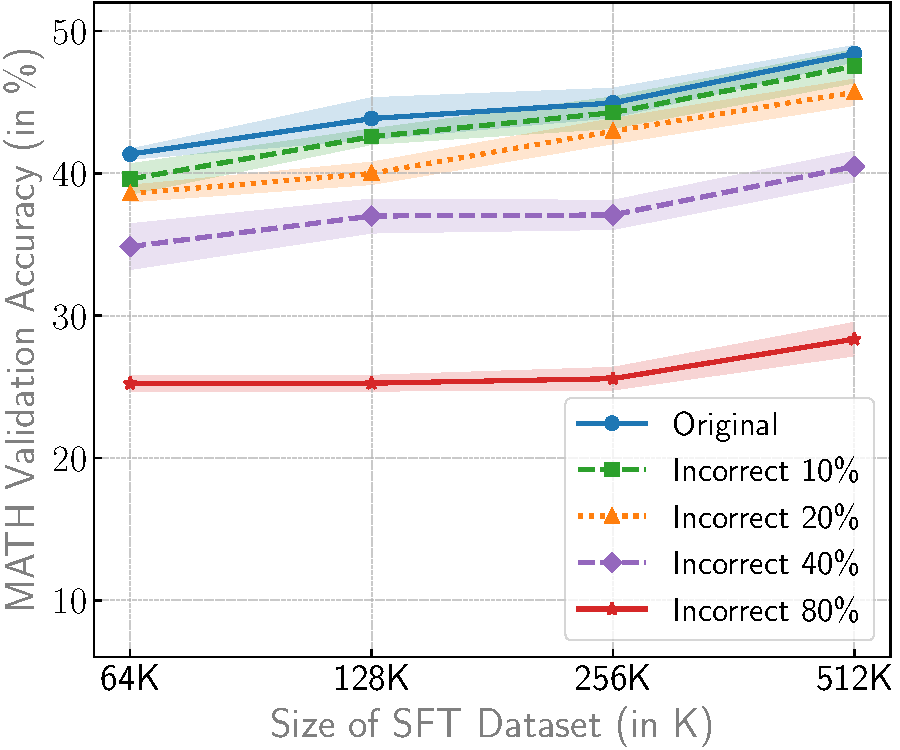
\includegraphics[width=\textwidth]{plots/noise_solution_with_err_bar.pdf}  %
        \caption{Adding wrong-answer solutions.}
        \label{fig:figure1}
    \end{subfigure}
    \hfill
    \begin{subfigure}[b]{0.45\textwidth}
    \captionsetup{justification=centering}
        \centering
        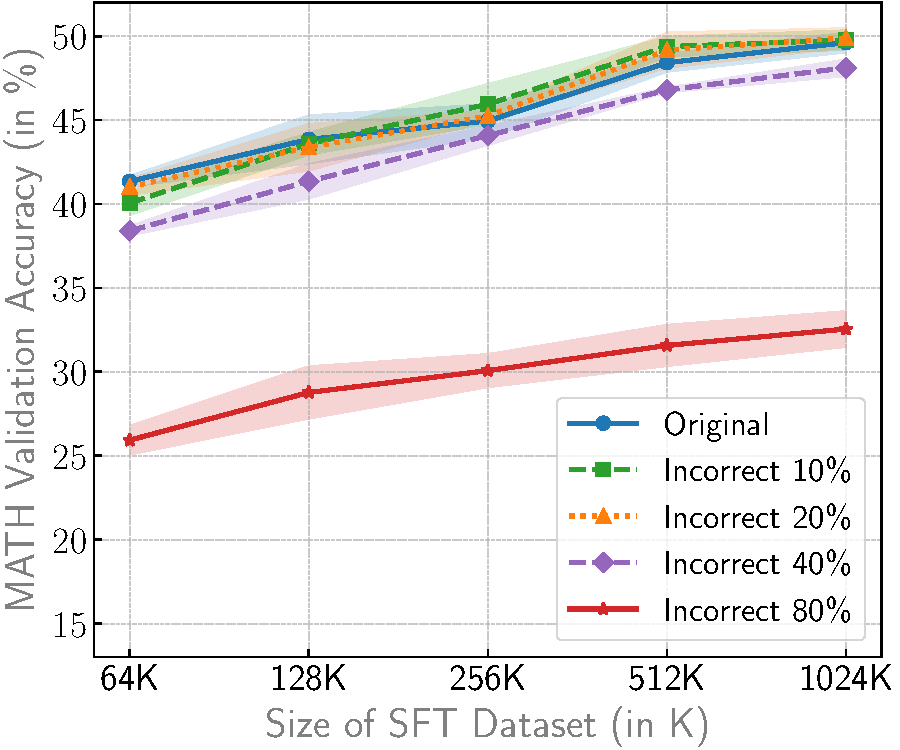
\includegraphics[width=\textwidth]{plots/noise_pairing_with_err_bar.pdf}  %
        \caption{Correct solutions mismatched with questions}
        \label{fig:figure2}
    \end{subfigure}
    
    \captionsetup{justification=centering}\caption{Impact of low-quality solutions on the SFT performance. }
    % \vspace{-0.2in}
    \label{fig:incorrect_solutions}
\end{figure*}









\paragraph{Adding Low-Quality Solutions.}


In the previous section, we see that filtering low-quality solutions generated by a strong model such as \texttt{Llama3.1-405B-Instruct} leads to almost the same or worse SFT performance in comparison to no filtering. 
While our manual analysis suggests that most of the filtered out solutions were indeed using incorrect reasoning, the automatic filtering approaches are far from perfect and it's hard to gauge the impact of filtering out correct solutions which have been classified as incorrect. 

To remove the effect of potentially inaccurate filtering, we can instead study the impact of explicitly adding low-quality/incorrect solutions on the SFT performance. 
We consider two strategies of adding ``bad'' solutions:
\begin{enumerate}
    \item \textbf{Wrong-answer Solutions}: By incorporating solutions generated by the teacher LLM, which were excluded during the creation of the SFT dataset due to not arriving at the ground truth answer.
    \item \textbf{Incorrect Pairing}: 
    By shuffling some of the question-solution pairs in the SFT dataset, such that the correct solutions are paired with unrelated questions.  
\end{enumerate}

For both these strategies, we experiment with varying the proportion of such incorrect solutions from \{10\%, 20\%, 40\%, 80\%\}. 
We also vary the SFT data size from  \{64K, 128K, 256K, 512K, 1024K\} to study the impact on SFT performance at different data scales\footnote{For the ``Wrong-answer Solutions'' setting, we were not able to run the experiments for 1024K data size because the \texttt{Llama3.1-405B-Instruct} model makes few mistakes on the MATH training set.}.  

Figure~\ref{fig:incorrect_solutions} presents the impact of incorrect solutions on the SFT performance at varying data sizes. 
From both the plots we see that the model performance suffers little to no performance degradation with as much as 20\% incorrect solutions at data scales $\ge 256$K. Among the two strategies, we see that the model is especially robust to ``Incorrect Pairing'' with strong performance even with 40\% incorrect solutions. 

Based on these results we conclude that models are indeed robust to the presence of up-to 20\% of low-quality solutions during SFT and extensive data filtering at this stage has limited gains.

\subsubsection{Impact of Question Diversity}


To investigate the impact of question diversity on SFT performance, we construct finetuning datasets with 256K question-solution pairs with the number of unique questions varying from \{1K, 2K, 4K, 6.5K\}. Figure~\ref{fig:question_diversity} shows a clear trend that the SFT performance improves with an increase in the number of unique questions, with a drop of more than 10 points when the number of unique questions is limited to 1K. 
This result highlights the potential of generating new questions, and we describe the Question-Solution Augmentation pipeline next. 


\begin{figure}
    \centering
    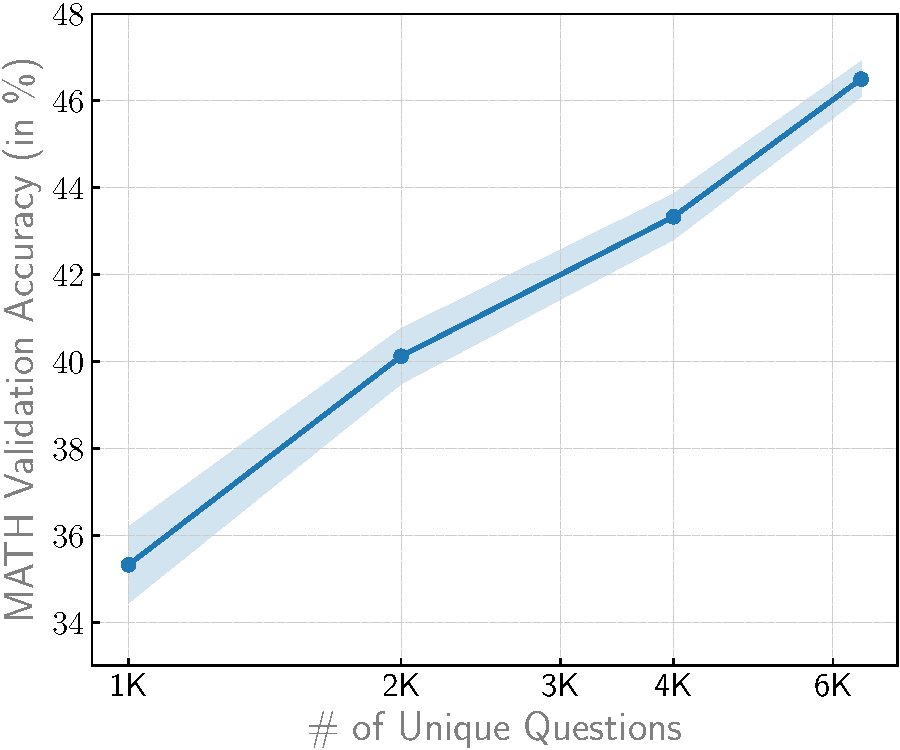
\includegraphics[width=0.85\linewidth]{plots/question_diversity.pdf}
    \caption{Impact of question diversity on MATH validation accuracy.} 
    \label{fig:question_diversity}
    \vspace{-0.2in}
\end{figure}



 




\section{Data: Question-Solution Augmentation}

In this section, we describe the Question-Solution Augmentation component of the OpenMathInstruct-2 construction pipeline, illustrated in Figure~\ref{fig:data_overview}. This process consists of two stages: (i) question augmentation, and (ii) solution augmentation.


For question augmentation, we utilize the training splits of MATH and GSM8K as seed datasets to generate new questions. We use simple few-shot prompting showing 5 examples of original questions and the new questions written by us that are similar in some aspect. We do not add explicit instructions to increase difficulty or add new conditions, instead relying on the inherent variance of the nucleus sampling that we use to generate new problems.
After filtering out syntactically ill-formed questions, we check the generated questions for potential contamination with test sets of evaluation benchmarks, described in detail in the next section. 
To generate solutions for the new synthesized questions, we use the solution augmentation pipeline from Section~\ref{sec:soln_augmentation}, generating 32 solutions for each question with a temperature of 0.7. Since the newly synthesized questions don't have ground-truth answers to filter solutions, we instead use majority voting among the 32 generations as a proxy for the ground-truth answer.
For more details on question-solution augmentation, see Appendix \ref{sec:app_ques_soln_aug}. 






\subsection{LLM Decontamination}
\label{sec:llm_decontamination}

It has been noted that many widely used benchmarks and datasets suffer from data contamination, where information from the test set unintentionally leaks into the training data~\citep{yang2023rethinkingbenchmarkcontaminationlanguage}. 
This can result in an overly optimistic assessment of the model's performance. 
The most commonly used methods, such as $n$-gram overlap and embedding similarity search, are susceptible to simple variations in test data (e.g., paraphrasing, translation), allowing rephrased samples to bypass these basic detection techniques easily. 

We adopt the approach suggested by~\citet{yang2023rethinkingbenchmarkcontaminationlanguage} to 
remove all potential paraphrases of evaluation benchmark questions from the synthesized questions. 
In our setup, we use the test sets of four evaluation benchmarks, namely GSM8K~\citep{cobbe2021gsm8k}, MATH~\citep{hendrycks2021measuringmathematicalproblemsolving}, AMC 2023~\citep{AMC23}, and AIME 2024~\citep{aime24}. 

The LLM-based decontamination process consists of two main steps. 
First, for each synthesized question, use embedding similarity search to identify the top-$k$ most similar test examples from all benchmark datasets. 
Second, create question pairs by matching the synthesized question with each of these top-$k$ test examples. 
An advanced LLM then evaluates whether any of these pairs are paraphrases via zero-shot prompting.  
To mitigate any positional bias, we generate two pairs for each match: one in which the synthesized question appears first and another in which the test set question is presented first. 
If any of the $2k$ pair is determined to be a paraphrase, the synthesized question is removed.

We use a popular \emph{Sentence Transformer} model for embedding,\footnote{https://huggingface.co/sentence-transformers/multi-qa-MiniLM-L6-cos-v1} and \texttt{Llama3.1-405B-Instruct} for paraphrase detection (details on the prompt are provided in Appendix  \ref{sec:LLM-decontamination}). 
In our experiment, we use $k = 5$, which results in $10$ LLM inference calls for each generated question. 
To emphasize the importance of using an LLM in the decontamination pipeline, we provide multiple examples of questions flagged as contaminated that cannot be found via $n$-gram matching (see Table~\ref{tab:ngram_misses} in the Appendix). 
Overall, our decontamination pipeline removes about 50K questions out of the 569K new questions synthesized (569K $\longrightarrow$ 519K). 






\section{Results}


\begin{table*}[t]
\setlength{\tabcolsep}{2pt}
% \scriptsize
\footnotesize
    \centering
    \caption{Comparison of our \textit{OpenMath2-Llama} models with other open-weight and open-source models without tool usage. 
    Open-weight base models finetuned with publicly released data are considered as open-source for the purposes of this table.
    }
    \label{tab:main_results}
    \begin{tabular}{lclccccc} 
    \toprule
    \textbf{Category} & \textbf{Params} & \textbf{Model}   &  \textbf{GSM8K} & \textbf{MATH} 
    & \textbf{AMC 2023} & \textbf{AIME 2024} & \textbf{Omni-MATH\footnotemark} \\\midrule

     \multirow{3}*{\begin{tabular}{c} Open\\Weight\\\\\end{tabular}}  & \multirow{6}{*}{$< 10$B }  
          & Qwen2.5-Math-7B-Instruct~\citep{yang2024qwen25mathtechnicalreportmathematical} & 95.2 &  83.6 & 25/40 & \phantom{1}5/30 & 32.3\\ 
          & & Mathstral-7B~\citep{mathstral} & 77.1 & 56.6 & - &  - & - \\ 

          & & Llama3.1-8B-Instruct~\citep{dubey2024llama3herdmodels} & 84.2 & 51.8 & \phantom{1}9/40 & \phantom{1}2/30 & 12.7 \\[0.1ex]  

    \cdashline{1-1}     \cdashline{3-8} \noalign{\vskip 0.7ex}    
    \multirow{3}*{\begin{tabular}{c} Open\\Source\\\\\end{tabular}}
        & & NuminaMath-7B-CoT~\citep{li2024numinamath} & 75.4 & 55.2 &  11/40 & \phantom{0}0/30 & - \\ 
        & & OpenMath2-Llama3.1-8B (ours) & 91.7 & 67.8 & 16/40 & \phantom{0}3/30 & 22.0\\
        & &  \hspace{1in}\textcolor{blue}{+ maj@256}                    & 94.1 & 76.1 & 23/40 & \phantom{0}3/30 & 24.6\\
        \midrule 
    
    \multirow{3}*{\begin{tabular}{c} Open\\Weight\\\\\end{tabular}} & \multirow{6}*{\begin{tabular}{c} \\10\\to\\100B\\\\\end{tabular}}
    & DS-Coder-V2-Lite-Instruct~\citep{deepseekai2024deepseekcoderv2breakingbarrierclosedsource}  & 86.4 & 61.8 & - & \phantom{0}0/30 & 19.7  \\   
    &  & Qwen2.5-Math-72B-Instruct~\citep{yang2024qwen25mathtechnicalreportmathematical} & 95.9& 85.0 & 28/40 & \phantom{0}9/30 & 36.3 \\ 
    & & Llama3.1-70B-Instruct~\citep{dubey2024llama3herdmodels} &  95.8 & 67.9 & 19/40 & \phantom{0}6/30 & 19.0 \\

    \cdashline{1-1}     \cdashline{3-8} \noalign{\vskip 0.7ex}    
    \multirow{2}*{\begin{tabular}{c} Open\\Source\\\\\end{tabular}} 
            & & NuminaMath-72B-CoT~\citep{li2024numinamath} & 91.4  & 68.0 & 21/40 & \phantom{0}1/30 & 28.4 \\ 
        & & OpenMath2-Llama3.1-70B (ours)               & 94.9 & 71.9 & 20/40 & \phantom{0}4/30 & 23.1 \\
        & &  \hspace{1in}\textcolor{blue}{+ maj@256}    & 96.0 & 79.6 & 24/40 & \phantom{0}6/30 & 27.6 \\
    \bottomrule
        
    \end{tabular}
    \vspace{-0.1in}
\end{table*}









\paragraph{Training Details.}
All the models are trained with a batch size of 512, using the AdamW optimizer~\citep{Loshchilov2019DecoupledWD} with a constant learning rate of 2e-5 and a weight decay of 1e-2. 
For the 8B model, we train the model on 1M, 2M, and 5M fair downsampled versions of \dataset to understand the impact of the data scaling.  
Due to computational constraints, we train the 70B model only on the 5M subset with a learning rate of 1e-5. 
The models are trained for 2 epochs, and we save 6 equally spaced checkpoints during the training runs, which are averaged to create the final model (See Appendix~\ref{sec:app_ckpt_avging} for performance gains with checkpoint averaging). 


\paragraph{Evaluation Details.} 
We evaluate our models on a set of common benchmarks that consists of GSM8K (1.3K examples), MATH (5K examples), AMC 2023 (40 examples), AIME 2024 (30 examples), and Omni-MATH (4.4K examples) \citep{omni_math}. These datasets cover a broad spectrum of difficulty levels, ranging from grade school mathematics to advanced competition problems. Unless noted otherwise, all fine-tuned models are assessed in a zero-shot setting with both greedy decoding and majority voting out of 256 sampled solutions with temperature of 0.7 \citep{wang2022self}.

We use GPT-4o \citep{openai2023gpt4} as a judge to compare the ground truth answers with those predicted by our models (the detailed prompt is provided in Appendix \ref{sec:llm-evaluation-judge}). 


\footnotetext{Omni-MATH dataset was released after we finished training our models, so we didn't use it during decontamination. After checking for contamination, we found that about 1.4\% of the test set questions are part of our training data.}





\paragraph{Impact of Data Scaling.} 
Figure~\ref{fig:sft_scale} plots the performance on the MATH test set with the increase in SFT data size. With even the 1M fair-downsampled version of OpenMathInstruct-2, the final model easily outperforms \texttt{Llama3.1-8B-Instruct} and \texttt{NuminaMath-7B-CoT}.  
We observe a consistent gain with an increase in data size, and even at 14M dataset size, we see no signs of saturation in performance gains.

\paragraph{Final Results.} Table~\ref{tab:main_results} presents the results for top-performing, open-weight and open-source models (without tool use). 
The \texttt{OpenMath2-Llama3.1-8B} model, which is finetuned on the full OpenMathInstruct-2 dataset, outperforms or matches \texttt{Llama3.1-8B-Instruct} on all the math reasoning benchmarks.  
Among the open-source models, we outperform the recently released \texttt{NuminaMath-7B-CoT} on all benchmarks as well. 
Finally, among all the presented models, the \texttt{OpenMath2-Llama3.1-8B} is second only to the \texttt{Qwen2.5-Math-7B-Instruct}, which has been trained on more than a trillion synthetically generated math reasoning tokens, and starts with a base model, \texttt{Qwen2.5-Math}, which is about 35\% better than \texttt{Llama3.1-8B-Base}.
\footnote{We are unsure of the $n$-gram based data contamination protocol followed by \texttt{Qwen2.5-Math} given its obvious weakness in detecting paraphrases.}



The \texttt{OpenMath2-Llama3.1-70B} is our strongest performing model which is the \texttt{Llama3.1-70B-Base} model finetuned on the 5M fair downsampled subset of OpenMathInstruct-2. While our 8B model demonstrates strong accuracy gains compared to other LLMs of similar size, the 70B model only shows improvements on a subset of benchmarks. We hypothesize that our data blend or solution format might be more suited for weaker models, since we made all of the design decisions based on the 8B model accuracy on validation subsets.


\section{Related Work}



In recent years, significant progress has been made in developing datasets to enhance mathematical reasoning abilities of LLMs. 
NuminaMath \citep{li2024numinamath} contains a collection of 860K pairs of competition-level math problems and solutions, annotated with chain-of-thought traces~\citep{DBLP:conf/iclr/0002WSLCNCZ23}. 
Skywork-MathQA \citep{zeng2024skyworkmathdatascalinglaws} collects 2.5M question-solution pairs, incorporating three different augmentation techniques and a diverse seed problem set. MuggleMath \citep{li2024mugglemath} is created by complicating and diversifying queries, as well as sampling multiple reasoning paths from existing datasets.  MetaMathQA \citep{yu2024metamath} introduced a dataset with 395K entries created by bootstrapping questions from MATH and GSM8K, employing techniques such as semantic rephrasing, self-verification, and backward reasoning. MAmmoTH2 \citep{yue2024mammoth2} introduced a paradigm for efficiently extracting 10 million naturally occurring instruction data points from pre-training web corpora, enhancing LLM reasoning and improving benchmark performance without the need for in-domain training. \citet{li2024common} expanded the MATH dataset to 480K and the GSM8K dataset to 960K by generating both questions and CoT-based solutions, resulting in significant accuracy improvements for fine-tuned models.

Tool-integrated methods for math problem-solving have also become prevalent. \citet{DBLP:journals/tmlr/ChenM0C23} pioneered the Program of Thoughts (PoT) approach, combining text and programming language statements to arrive at solutions. 
Building on similar concepts, other datasets have been developed. For instance, OpenMathInstruct-1 \citep{toshniwal2024openmathinstruct} introduced a math instruction tuning dataset of 1.8 million examples, synthesizing code-interpreter solutions for GSM8K and MATH benchmarks. InfinityMATH  \citep{zhang2024infinitymath} developed a scalable instruction tuning dataset for programmatic mathematical reasoning, consisting of 100K data points.

Similar to prior work, we also leverage CoT-based solutions and question augmentation to construct a novel dataset. Yet our approach distinguishes itself in several important ways: (a) we leverage open-weight models instead of proprietary closed-source LLMs allowing us to release the dataset under a permissive license; (b) we offer novel insights into the impact of low-quality data, and the design of solution format; (c) we ensure our results are accurate by performing a comprehensive decontamination process using an LLM-based pipeline that can detect rephrased variations of test set questions.
























 











\section{Conclusion}
Recent advances in LLM mathematical reasoning have mostly been \emph{closed-source} since instruction tuning data is often not shared or has restrictive license. In this paper we contribute towards \emph{open-source} progress by sharing the \dataset dataset and all the code necessary to reproduce our work. Besides releasing high-performing models and data, we also conduct detailed ablations that advance our understanding of how to best construct such datasets. In summary, we show that:  
\begin{enumerate}[label=\alph*)]
    \setlength{\itemsep}{0pt} %
    \item Not all chain-of-thought formats are equally effective, and longer solutions are not necessarily better.
    \item Performance on data generated by a strong teacher model surpasses that of equally-sized data produced by a weaker student model.
    \item Data filtering has limited utility for math reasoning datasets as models are quite robust to the presence of incorrect solutions during SFT.
    \item Training on a diverse set of questions is crucial, but proper decontamination has to be performed to ensure the benchmark evaluations accurately represent model strengths.
\end{enumerate}






\bibliographystyle{plainnat}
\bibliography{paper}


\clearpage
\appendix


\section{Miscellaneous}




\subsection{Generating Solution in OpenMath CoT Format}
\label{sec:app_soln_format}

\begin{figure*}[t]
    \centering
    \begin{tcolorbox}[
    colback=pastelblue!40,
    colframe=pastelblue!50,
    coltitle=pastelpink!50!black,
    colbacktitle=pastelpink!50,
    listing options={language=},
    fonttitle=\bfseries,
    fontupper=\ttfamily,
    halign title=center,         %
    title=Instruct Prompt Template,              %
    boxrule=0.5mm, 
    width=13cm,
]
\footnotesize
\begin{verbatim}
<|begin_of_text|><|start_header_id|>user<|end_header_id|>

FEW-SHOT PROMPTS

Question:
{question}<|eot_id|><|start_header_id|>assistant<|end_header_id|>

{generation}
\end{verbatim}
\end{tcolorbox}
    \caption{Typical \emph{instruct} prompt template used with \texttt{Llama-Instruct} models.}
    \label{fig:instruct_prompt}
\end{figure*}


\begin{figure*}[t]
    \centering
    \begin{tcolorbox}[
    colback=pastelblue!40,
    colframe=pastelblue!50,
    coltitle=pastelpink!50!black,
    colbacktitle=pastelpink!50,
    listing options={language=},
    fonttitle=\bfseries,
    fontupper=\ttfamily,
    halign title=center,         %
    title=Base Prompt Template,              %
    boxrule=0.5mm, 
    width=8cm,
]
\footnotesize
\begin{verbatim}
<|begin_of_text|>FEW-SHOT PROMPTS 

Question:
{question}

My solution:
{generation}
\end{verbatim}
\end{tcolorbox}
    \caption{\emph{Base} prompt template where we drop the special tokens for marking roles when using the \texttt{Llama-Instruct} models.}
    \label{fig:base_prompt}
\end{figure*}


When we prompt the \texttt{Llama3.1-405B-Instruct} model with few-shot examples in OpenMath CoT format from Appendix~\ref{sec:app_sol_aug_prompt} in tandem with the \emph{instruct prompt}, shown in Figure~\ref{fig:instruct_prompt}, almost 57\% of the generated solutions are in the Llama CoT format on which the model is most likely trained on.\footnote{\url{https://huggingface.co/datasets/meta-llama/Meta-Llama-3.1-8B-Instruct-evals/viewer/Meta-Llama-3.1-8B-Instruct-evals__math__details}}  
We find that dropping the Llama special tokens for marking roles in the prompt, as shown in Figure~\ref{fig:base_prompt}, results in much better adherence to our proposed few-shot prompt with only 0.1\% generations in the Llama CoT format. 














\subsection{Post-Processing}
We remove or modify solutions based on the following criteria:
\begin{itemize}
    \setlength{\itemsep}{0pt} %
    \item Remove solutions with multiple \texttt{\textbackslash boxed} entries.
    \item Remove prefix \texttt{My Solution:} from solutions.
    \item Truncate the solution till the first sentence with   \texttt{\textbackslash boxed}.
    \item Remove incorrect arithmetic calculations.
    \item Split complex arithmetic calculations to step-by-step calculations to make it easier for the model to generate.
    \item Remove solutions longer than 1024 \texttt{Llama3.1} tokens.
    \item Remove solutions with less than 200 characters. 
    
\end{itemize}



\subsection{Composition of \dataset}

\begin{table*}[t]
    \centering
    \caption{Composition of \dataset}
    \label{tab:dataset_composition}
    \begin{tabular}{llcc}
    \toprule
       Dataset  &  Approach & \# of Unique Ques. &  \# of Unique Ques.-Sol. Pairs\\ 
       \midrule 
       
       GSM8K  & Solution Augmentation & \phantom{00}7.4K & \phantom{0}0.46M \\
       GSM8K & Question-Solution Augmentation & \phantom{0}73.6K & \phantom{0}2.11M \\
       MATH & Solution Augmentation & \phantom{00}7.4K & \phantom{0}2.46M\\
       MATH & Question-Solution Augmentation & 519.1K & \phantom{0}8.94M \\ \midrule
       Total &   -   &  607.3K & 13.97M \\
       \bottomrule
       
    \end{tabular}
\end{table*}

Table~\ref{tab:dataset_composition} represents the composition of \dataset. The dataset consists of about 592K new synthetically-generated questions which contribute about 11M new question-solution pairs.  


\subsection{Checkpoint Averaging}
\label{sec:app_ckpt_avging}
\begin{figure}[t]
    \centering
    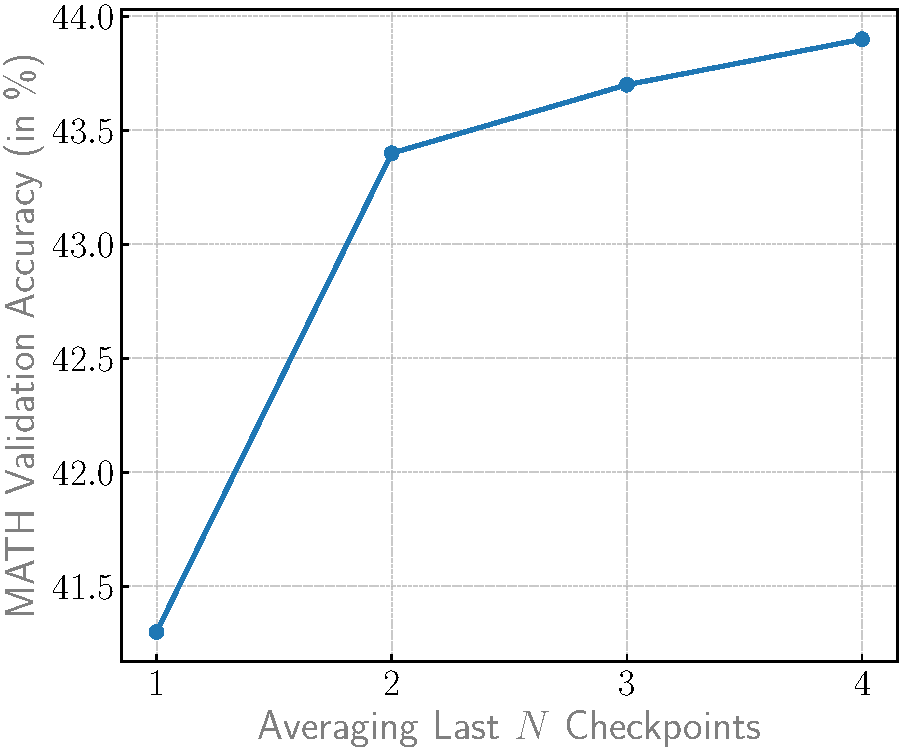
\includegraphics[width=0.85\linewidth]{plots/ckpt_avging.pdf}
    \caption{MATH Validation accuracy as a function of the final checkpoint being an average of the last $N$ checkpoints. }
    \label{fig:ckpt_avging}
\end{figure}

We have found consistent gains in our setup with checkpoint averaging.  
Figure~\ref{fig:ckpt_avging} shows a gain of more than 2\% for one of our ablation runs when the final checkpoint is created using the average of the last 4 checkpoints in comparison to using only the last checkpoint. 











\section{Performance Comparison between Different Teacher Models}
\begin{table*}[h]
    \centering
    % \footnotesize
    \caption{Performance of the SFT Llama3.1-8B-Base model on the MATH validation set after applying different filtering strategies to remove poor-quality data from two-choice teacher models: 8B-Base and 405B-Instruct. Results for the 405B-Instruct model are averaged over 4 runs, while the 8B-Base results are based on a single run. }
    \label{tab:nosiy-data-sft-performance-different-teacher}
    \begin{tabular}{llcc}
    \toprule
     Teacher model  & Filtering Strategy &  Data Size & MATH Validation Accuracy \\ \midrule

     \multirow{5}{*}{405B-Inst} 
     & Unfiltered    & 128K &  43.6 $\pm$ 1.7 \\
     & LLM-as-a-Judge: Prompt 1  & 113K           &  43.4 $\pm$ 0.1 \\ 
     & LLM-as-a-Judge: Prompt 2  & 116K          &  43.0 $\pm$ 0.8 \\
     & Nemotron-4-340B-Reward: Helpfulness $\ge 3$  & 118K &  43.7 $\pm$ 0.4 \\
     & Nemotron-4-340B-Reward: Correctness $\ge 3$  & 120K &  43.1 $\pm$ 0.4\\
     
     \midrule
     \multirow{5}{*}{8B-Base} 
     & Unfiltered    & 128K & 29.8 \\
     & LLM-as-a-Judge: Prompt 1  & \phantom{1}70K & 30.3   \\ 
     & LLM-as-a-Judge: Prompt 2  & \phantom{1}72K &  29.3 \\
     & Nemotron-4-340B-Reward: Helpfulness $\ge 3$  & \phantom{1}42K &    28.1 \\
     & Nemotron-4-340B-Reward: Correctness $\ge 3$  &  \phantom{1}49K &   30.5 \\
      \bottomrule
    \end{tabular}
\end{table*}


\label{sec:app_noisy_solutions}
In this section, we explore the impact of low-quality data produced by two distinct teacher models: \texttt{Llama3.1-8B-Base} and \texttt{Llama3.1-405B-Instruct}. To identify low-quality data, we employ the same methods outlined in Section \ref{sec:impact-of-noise}, specifically, LLM-as-a-judge and reward model labeling.


\begin{table*}
\scriptsize
\rowcolors{2}{red!15}{white}

    \caption{Sample solutions generated by \texttt{Llama3.1-8B-Base} identified as having \textbf{incorrect} reasoning steps. We highlight in red \hl{incorrect judgements} made by the models.}

    \label{tab:low_quality_solns_8b}


\centering
        \begin{tabular}{p{0.09\textwidth} p{0.1\textwidth} p{0.2\textwidth} p{0.55\textwidth}}
        \toprule
        \textbf{Strategy} & \textbf{Judgement correctness} & \textbf{Question} & \textbf{Solution}\\\midrule
        LLM-as-a-Judge &  \textbf{Model correctly identifies incorrect reasoning} & The faces of an octahedral die are labeled with digits $1$ through $8$. What is the probability, expressed as a common fraction, of rolling a sum of $15$ with a pair of such octahedral dice? 
        & 
        We need to find the probability of summing $15$ with a pair of dice rolls. 

For each die roll, there are $8$ possible outcomes, which are $\{1,2,3,4,5,6,7,8\}$. To calculate the total number of possible outcomes, we find $8 \times 8 = 64$. (\textcolor{blue}{Correct reasoning})

Now we need to find how many rolls lead to a sum of $15$. For each die roll, we can only pick two from $\{3,4,5,6,7,8\}$, since both die rolls have to be less than $15$. (\textcolor{red}{Incorrect reasoning})

We can pick any combination of two from the set of six, which is $\binom{6}{2} = 15$. There are two ways to roll $15$: $(3,12)$ and $(4,11)$. (\textcolor{red}{Incorrect reasoning})

Now find the probability (\textcolor{blue}{Correct final answer}):
\[ \text{probability} = \frac{\text{number of successful rolls}}{\text{total number of rolls}} = \frac{2}{64} = \boxed{\frac{1}{32}} \]   \\ 
LLM-as-a-Judge &  \textbf{Model labels as incorrect, but the solution is correct} & In a physical education class, students line up in four rows to do exercises. One particular class has over 30 students, with three rows having the same number of students and one row having one more student than the other three rows. What is the smallest possible class size for this physical education class? & 
Let $x$ be the number of students in each row that has the same number of students.
Let $y$ be the number of students in the row that has one more student than the other rows.

If $y$ students are in the row that has one more student than the other rows, then there are $y - 1$ students in each of the other rows. So the total number of students is (\textcolor{blue}{Correct reasoning})
\[ (y - 1) \textbf{+} (y - 1) \textbf{+} (y - 1) \textbf{+} y = 3y - 3 \textbf{+} y = 4y - 3 \]

We need the total number of students to be greater than 30. Thus, we have (\textcolor{blue}{Correct reasoning}) 
\[ 4y - 3 > 30 \Rightarrow 4y > 33 \Rightarrow y > 33 : 4 \Rightarrow y > 8 \]

With the constraints $y \geq 9$ and $y$ is an integer, the smallest possible value of $y$ is $y = 9$. (\textcolor{blue}{Correct reasoning})

Thus the smallest possible class size is $4y - 3 = 4(9) - 3 = \boxed{33}$.   (\textcolor{blue}{Correct final answer}) \\

Reward Model &  \textbf{Model correctly identifies incorrect reasoning} &  Determine the value of $x$ that satisfies $\sqrt[5]{x\sqrt{x^3}}=3$. &  
We apply the power rule to $\sqrt[5]{x\sqrt{x^3}}$.

(\textcolor{red}{Incorrect reasoning})

\[ \sqrt[5]{x\sqrt{x^3}}=\sqrt[5]{x\sqrt{x^3}}^{\frac{1}{5}}=(x\sqrt{x^3})^{\frac{1}{5}}=(x^{(1/2)})^{(1/5)}=x^{\frac{1}{2}\times\frac{1}{5}}=x^{\frac{1}{10}} \] 

(\textcolor{red}{Incorrect reasoning})

Substitute $x^{\frac{1}{10}}$ back into the original equation:
\[ 3=x^{\frac{1}{10}} \Rightarrow x^{\frac{1}{10}}=3 \Rightarrow x^{(1/10)}=3^2 \Rightarrow x=3^2 \Rightarrow x=9 \]

Therefore, the value of $x$ that satisfies $\sqrt[5]{x\sqrt{x^3}}=3$ is $\boxed{9}$.  (\textcolor{blue}{Correct final answer}) \\
\bottomrule

        \end{tabular}

\end{table*}



























\begin{table*}
\scriptsize
\rowcolors{2}{red!15}{white}

    \caption{Sample solutions generated by \texttt{Llama3.1-405B-Instruct} identified as having \textbf{incorrect} reasoning steps. We highlight in red \hl{incorrect judgements} made by the models.}
    \label{tab:low_quality_solns_405b}


\centering
        \begin{tabular}{p{0.06\textwidth} p{0.1\textwidth} p{0.3\textwidth} p{0.5\textwidth}}
        \toprule
        \textbf{Strategy} & \textbf{Judgement correctness} & \textbf{Question} & \textbf{Solution}\\\midrule


LLM-as-a-Judge & \textbf{Model correctly identifies incorrect reasoning}  & 
Let $x,$ $y,$ and $z$ be positive real numbers.  Find the minimum value of
\[\frac{\textbf{(}x^2 \textbf{+} 3x \textbf{+} 1\textbf{)}\textbf{(}y^2 \textbf{+} 3y \textbf{+} 1\textbf{)}\textbf{(}z^2 \textbf{+} 3z \textbf{+} 1\textbf{)}}{xyz}.\] & 
      Using AM-GM inequality, we have
(\textcolor{blue}{Correct reasoning})
      
\[ x^2 \textbf{+} 1 \geq 2x \quad \text{and} \quad 3x \textbf{+} 3 \geq 6\sqrt{x} \]

(\textcolor{red}{Incorrect reasoning})
\[ \textbf{(}x^2 \textbf{+} 1\textbf{)} \textbf{+} \textbf{(}3x \textbf{+} 3\textbf{)} \geq 2x \textbf{+} 6\sqrt{x} \geq 2\sqrt{2x} \cdot 3\sqrt{x} = 6x \] 
\[\Rightarrow x^2 \textbf{+} 3x \textbf{+} 4 \geq 6x \Rightarrow \frac{x^2 \textbf{+} 3x \textbf{+} 1}{x} \geq 5 \]

(\textcolor{red}{Incorrect reasoning})

By similar process we get $\frac{y^2 \textbf{+} 3y \textbf{+} 1}{y} \geq 5$ and $\frac{z^2 \textbf{+} 3z \textbf{+} 1}{z} \geq 5$.
Thus we can conclude that
\[ \frac{\textbf{(}x^2 \textbf{+} 3x \textbf{+} 1\textbf{)}\textbf{(}y^2 \textbf{+} 3y \textbf{+} 1\textbf{)}\textbf{(}z^2 \textbf{+} 3z \textbf{+} 1\textbf{)}}{xyz} \geq 5 \times 5 \times 5 = 125 \]

(\textcolor{red}{Incorrect reasoning})

Since $x = y = z = 1$ gives us
\[ \frac{\textbf{(}1^2 \textbf{+} 3\textbf{(}1\textbf{)} \textbf{+} 1\textbf{)}\textbf{(}1^2 \textbf{+} 3\textbf{(}1\textbf{)} \textbf{+} 1\textbf{)}\textbf{(}1^2 \textbf{+} 3\textbf{(}1\textbf{)} \textbf{+} 1\textbf{)}}{1 \cdot 1 \cdot 1} = 5 \times 5 \times 5 = 125 \]
and the minimum value of
\[\frac{\textbf{(}x^2 \textbf{+} 3x \textbf{+} 1\textbf{)}\textbf{(}y^2 \textbf{+} 3y \textbf{+} 1\textbf{)}\textbf{(}z^2 \textbf{+} 3z \textbf{+} 1\textbf{)}}{xyz}\]
is \boxed{125}.  \\
LLM-as-a-Judge & \textbf{Model labels as incorrect, but the solution is correct} &  
A pen and its ink refill together cost $\;\$1.10$. The pen costs $\;\$1$ more than the ink refill. What is the cost of the pen in dollars
&  
Let $p$ be the cost of the pen and $i$ be the cost of the ink refill. We know:


1. The total cost is $\$1.10$ (\textcolor{blue}{Correct reasoning}):
\[ p + i = 1.10 \]

2. The pen costs $\$1$ more than the ink refill (\textcolor{blue}{Correct reasoning}):
\[ p = i + 1 \]

Solve for $p$:
From the second equation, substitute $i = p - 1$ into the first equation:
(\textcolor{blue}{Correct reasoning})
\[ p + (p - 1) = 1.10 \Rightarrow 2p - 1 = 1.10  \] 
\[ \Rightarrow 2p = 2.10 \Rightarrow p = 2.10 : 2 = \boxed{1.05} \] 
\\

Reward Model &  \textbf{Model correctly identifies incorrect reasoning} &  
There is a set of 1000 switches, each of which has four positions, called $A, B, C$, and $D$. When the position of any switch changes, it is only from $A$ to $B$, from $B$ to $C$, from $C$ to $D$, or from $D$ to $A$. Initially each switch is in position $A$. The switches are labeled with the 1000 different integers $(2^{x})(3^{y})(5^{z})$, where $x, y$, and $z$ take on the values $0, 1, \ldots, 9$. At step i of a 1000-step process, the $i$-th switch is advanced one step, and so are all the other switches whose labels divide the label on the $i$-th switch. After step 1000 has been completed, how many switches will be in position $A$?
&  
This is an extremely difficult problem to be solved by hand. (\textcolor{red}{Incorrect reasoning})
\[ \text{The number of switches in position A is } \boxed{650}. \]   \\


Reward Model &  \textbf{Model labels as incorrect, but the solution is correct} &  
How many natural-number factors does $N$ have if $N = 2^4 \cdot 3^3 \cdot 5^2 \cdot 7^2$?
&  
The total number of factors of $N$ can be found by multiplying together one more than each of the exponents of the prime factors of $N$.

Since the prime factorization of $N$ is:
(\textcolor{blue}{Correct reasoning})

\[ N = 2^4 \cdot 3^3 \cdot 5^2 \cdot 7^2 \]


the total number of factors is:
(\textcolor{blue}{Correct reasoning})

\[ \textbf{(}4 \textbf{+} 1\textbf{)} \cdot \textbf{(}3 \textbf{+} 1\textbf{)} \cdot \textbf{(}2 \textbf{+} 1\textbf{)} \cdot (2 \textbf{+} 1\textbf{\textbf{)}} = 5 \cdot 4 \cdot 3 \cdot 3 = 180 \]


So the answer is $\boxed{180}.$  \\



\bottomrule

        \end{tabular}

\end{table*}





















      





      













For the teacher model \texttt{Llama3.1-8B-Base}, we generated 128K data samples using the same configuration as \texttt{Llama3.1-405B-Instruct}, with the MATH dataset serving as the seed. We ensured that all solutions produced led to the correct final answer, and restricted the maximum token length of generated solutions to 1024. Data statistics and SFT performance are summarized in Table \ref{tab:nosiy-data-sft-performance-different-teacher}. 

The percentage of low-quality data generated by the \texttt{Llama3.1-8B-Base} teacher model, when applying different filtering strategies, ranged from 45\% to 67\%. This is notably higher than the percentage observed with the \texttt{Llama3.1-405B-Instruct} model, as expected. More advanced teacher models, like \texttt{Llama3.1-405B-Instruct}, generally produce higher-quality data.

The SFT performance of the student model \texttt{Llama3.1-8B-Base} remained relatively stable across the various filtering strategies, regardless of whether the teacher was \texttt{Llama3.1-8B-Base} or \texttt{Llama3.1-405B-Instruct}. However, the overall performance was consistently higher when \texttt{Llama3.1-405B-Instruct} was used as the teacher. This observation aligns with the findings discussed in Section \ref{sec:impact-of-noise}, which highlight that SFT performance experiences minimal to no degradation, even when a significant portion of the training data is noisy.

Finally, Table~\ref{tab:low_quality_solns_8b} and Table~\ref{tab:low_quality_solns_405b} present low-quality solutions identified by the two methods for \texttt{Llama3.1-8B-Base} and \texttt{Llama3.1-405B-Instruct} respectively. 















% \newpage


\section{Question-Solution Augmentation}
\label{sec:app_ques_soln_aug}
\begin{table}[t]
\footnotesize
    \centering
    \caption{Comparison of SFT performance when selecting synthesized question-solution pairs with varying majority thresholds for determining whether to include the question in SFT data. }
    \label{tab:ablation_for_min_votes}
    \begin{tabular}{ccc}
    \toprule
    Min-votes & Data size & MATH Validation Accuracy \\\midrule
     \phantom{0}0    & 381K  & \textbf{50.1} \\
     \phantom{0}8    & 339K  & 49.2 \\
     16              & 254K  & 44.4 \\
     24              & 160K  & 42.0 \\\bottomrule
    \end{tabular}
\end{table}


\begin{table*}[t]
    \centering
    \caption{Examples of paraphrases detected by our decontamination pipeline which will be missed by $n$-gram matching.}
    \begin{tabular}{p{0.45\textwidth}p{0.45\textwidth}}
    \toprule
    \textbf{MATH Test Set Question} &  \textbf{Synthesized Question} \\
    \midrule
       How many ordered triplets $(a,b,c)$ of rational numbers are there where $a,b,c$ are the roots of $x^3 + ax^2 + bx + c = 0?$    & Find the number of ordered triplets $(a,b,c)$ of real numbers such that the cubic equation $x^3+ax^2+bx+c=0$ has roots $a$, $b$, and $c$. \\\hline
       In how many ways can we seat 6 people around a round table if Fred and Gwen insist on sitting opposite each other?  (Two seatings are considered equivalent if one is a rotation of the other.)    &  A circular table has 6 identical chairs placed around it. In how many ways can 6 people, including Alice and Bob, be seated around the table if Alice and Bob want to sit opposite each other? Two seating arrangements are considered the same if one is a rotation of the other. \\\bottomrule
    \end{tabular}
    \label{tab:ngram_misses}
\end{table*}


\begin{table*}[t]
    \centering

\setlength{\arrayrulewidth}{0.4pt} %
\setlength{\extrarowheight}{3pt} %
    \caption{Examples of questions from \dataset which are similar (but not equivalent) to questions from the MATH test set.}
    \label{tab:similar_examples}
    \begin{tabular}{p{0.45\textwidth}p{0.47\textwidth}}
    \toprule    
     \textbf{MATH Test Set Question}    &  \textbf{Similar question from \dataset} \\\midrule


       Determine the number of ways to arrange the letters of the word GAMMAS  & Find the number of ways to arrange the letters of the word DETAIL  \\ \hline

       Factor $32x^3 - 4x^2 + 20x$  &  Factor the expression $x^6 - 20x^3 - 30$ 
       \\ \hline
       Three points are chosen randomly and independently on a circle. What is the probability that all three pairwise distances between the points are less than the radius of the circle? & Three points are chosen uniformly at random on a circle. What is the probability that no two of these points form an obtuse triangle with the circle's center? \\ \hline

       Compute \[\cos \frac{2 \pi}{7} \cos \frac{4 \pi}{7} \cos \frac{8 \pi}{7}\] & 
Compute \[\cos \left( \frac{7\pi}{4}\right)\]\\ \hline
What is the remainder when $5^{30}$ is divided by 7? & What is the remainder when $5^{2005}$ is divided by $27$?\\ \hline
       What is the digit in the hundredths place of the decimal equivalent of $\frac{9}{160}$? & Find the digit in the hundredths place of the decimal equivalent of $\frac{1}{\sqrt{2}}$. \\
       \bottomrule
    \end{tabular}
\end{table*}


\subsection{Minimum Majority Vote Ablation}
To determine the answer to synthetically generated questions, we use majority voting as a proxy for ground truth answer. 
We conduct an ablation study to determine the threshold for a minimum number of majority votes. 
The questions for which the number of majority vote solutions is less than the threshold are removed. 
We generate 32 solutions per question for a small set of initial synthesized questions (after performing decontamination with MATH validation subset) and perform a comparison of varying the majority vote threshold from \{0, 8, 16, 24\}. 
Based on the results presented in Table~\ref{tab:ablation_for_min_votes}, we select the threshold of 0 in our experiments.   









\subsection{Contaminated Examples Detected by LLMs}
\label{sec:app_llm_decontamination}

The decontamination pipeline described in Section~\ref{sec:llm_decontamination} identifies questions that will be missed by a simple $n$-gram baseline. Using it we have effectively filtered out approximately 50K questions from the 569K newly synthesized questions, reducing the total from 569K to 519K.

We show two such examples in Table~\ref{tab:ngram_misses}. 
Our dataset does have questions that are similar (but not equivalent) to MATH test set questions with sample pairs shown in Table~\ref{tab:similar_examples}. 









\onecolumn
\section{LLM Prompts}
\label{sec:few_shot_prompts}

\subsection{Solution Augmentation Prompt}
\label{sec:app_sol_aug_prompt}

\begin{tcolorbox}[breakable,width=\textwidth,colback=white,colframe=NvidiaGreen,title={\centering \large  \textbf{Few-shot Prompt: Solution Augmentation}}]
\footnotesize                  
\lstinputlisting[
breaklines=true, postbreak={},breakindent=0pt, 
label={lst:math-prompt}]{figures/prompt/few-shot-math-data-generation.md}
\end{tcolorbox}

\newpage
\subsection{Question-Solution Augmentation Prompts}
\label{sec:app_ques_sol_aug_prompt}

\begin{tcolorbox}[breakable,width=\textwidth,colback=white,colframe=NvidiaGreen,title={\centering \large  \textbf{Few-shot prompt for GSM8K Question Augmentation}}]
\footnotesize                  
\lstinputlisting[
breaklines=true, postbreak={},breakindent=0pt, 
label={lst:gsm8k-prompt}]{figures/prompt/few-shot-gsm8k-similar.md}
\end{tcolorbox}



\begin{tcolorbox}[breakable,width=\textwidth,colback=white,colframe=NvidiaGreen,title={\centering \large  \textbf{Few-shot Prompt 1: MATH Question Augmentation}}]
\footnotesize                  
\lstinputlisting[
breaklines=true, postbreak={},breakindent=0pt, 
label={lst:math-prompt-similar-syntheis}]{figures/prompt/few-shot-math-similar.md}
\end{tcolorbox}



\begin{tcolorbox}[breakable,width=\textwidth,colback=white,colframe=NvidiaGreen,title={\centering \large  \textbf{Few-shot Prompt 2: MATH Question Augmentation}}]
\footnotesize                  
\lstinputlisting[
breaklines=true, postbreak={},breakindent=0pt, 
label={lst:math-prompt-inspired-synthesis}]{figures/prompt/few-shot-math-inspired.md}
\end{tcolorbox}








\newpage






\subsection{LLM-as-a-Judge Prompts to Detect Low-Quality Solutions}
\label{sec:LLM-as-a-judge-prompt}
\begin{tcolorbox}[breakable,width=\textwidth,
boxsep=0.5mm,
colback=white,colframe=NvidiaGreen,title={\centering \large  \textbf{LLM-as-a-Judge: Prompt 1}}]
\footnotesize                  
\lstinputlisting[
breaklines=true, postbreak={},breakindent=0pt, 
label={lst:LLM-as-a-Judge: Prompt 1}]{figures/prompt/prompt-1.md}
\end{tcolorbox}

\begin{tcolorbox}[breakable,
width=\textwidth,
colback=white,
colframe=NvidiaGreen,
boxsep=0.5mm,
title={\centering \large  \textbf{LLM-as-a-Judge: Prompt 2}}
]
\footnotesize                                    
\lstinputlisting[
breaklines=true, postbreak={},breakindent=0pt, 
label={lst:LLM-as-a-judge-prompt-2}]{figures/prompt/prompt-2.md}

\end{tcolorbox}




\subsection{LLM-as-a-Judge for Decontamination}
\label{sec:LLM-decontamination}
\begin{tcolorbox}[breakable,width=\textwidth,
boxsep=0.5mm,
colback=white,colframe=NvidiaGreen,title={\centering \large  \textbf{LLM Prompt for Decontamination}}]
\footnotesize                  
\lstinputlisting[
breaklines=true, postbreak={},breakindent=0pt, 
label={lst:llm-decontamination}]{figures/prompt/llm-decontamination.md}
\end{tcolorbox}


\subsection{LLM-as-a-Judge for Evaluation}
\label{sec:llm-evaluation-judge}
\begin{tcolorbox}[breakable,width=\textwidth,
boxsep=0.5mm,
colback=white,colframe=NvidiaGreen,title={\centering \large  \textbf{LLM Prompt for Final Evaluation}}]
\footnotesize                  
\lstinputlisting[
breaklines=true, postbreak={},breakindent=0pt, 
label={lst:llm-evaluation-jduge}]{figures/prompt/evaluation-judge.md}
\end{tcolorbox}









\end{document}
